\documentclass[10pt]{beamer}

\usetheme[progressbar=frametitle]{metropolis}
\usepackage{appendixnumberbeamer}
\usepackage[utf8]{inputenc}
\usepackage{booktabs}
\usepackage[scale=2]{ccicons}
\usepackage{xcolor}
\usepackage{pgfplots}
\usepgfplotslibrary{dateplot}
\usepackage{xspace}


\usepackage{listings}


% Emulate markdown's light grey background for monospace.
\usepackage{soul}
\definecolor{Light}{gray}{.96}
\sethlcolor{Light}
\let\OldTexttt\texttt
\renewcommand{\texttt}[1]{\OldTexttt{\hl{#1}}}% will affect all \texttt


%  Use knitr's colorscheme.
\definecolor{fgcolor}{rgb}{0.345, 0.345, 0.345}
\definecolor{hlnum}{rgb}{0.686,0.059,0.569}
\definecolor{hlstr}{rgb}{0.192,0.494,0.8}
\definecolor{hlcom}{rgb}{0.678,0.584,0.686}
\definecolor{hlopt}{rgb}{0,0,0}
\definecolor{hlstd}{rgb}{0.345,0.345,0.345}
\definecolor{hlkwa}{rgb}{0.161,0.373,0.58}
\definecolor{hlkwb}{rgb}{0.69,0.353,0.396}
\definecolor{hlkwc}{rgb}{0.333,0.667,0.333}
\definecolor{hlkwd}{rgb}{0.737,0.353,0.396}
\definecolor{shadecolor}{rgb}{0.969, 0.969, 0.969}

\lstset{
  backgroundcolor=\color{shadecolor},
  basicstyle=\color{hlstd}\sffamily\footnotesize,
  breakatwhitespace=false,
  %breaklines=true,
  captionpos=b,
  commentstyle=\color{hlcom},
  deletekeywords={...},
  escapeinside={\%*}{*)},
  extendedchars=true,
  frame=lines,
  keepspaces=true,
  keywordstyle=\color{hlkwb},
  morekeywords={*,...},
  numbers=left,
  numbersep=5pt,
  numberstyle=\tiny\color{hlstd},
  rulecolor=\color{hlstd},
  showspaces=false,
  showstringspaces=false,
  showtabs=false,
  stepnumber=1,
  stringstyle=\color{hlstr},
  tabsize=2,
  title=\lstname
}

\newcommand{\themename}{\textbf{\textsc{metropolis}}\xspace}

\title{KodeKlubben 2.0}
\subtitle{Øvelsesgang 2}
% \date{\today}
\date{\today}
\author{Kristian Urup Olesen Larsen, Jakob Jul Elben}
\institute{Økonomisk Institut, KU}
% \titlegraphic{\hfill\includegraphics[height=1.5cm]{logo.pdf}}

\begin{document}

\maketitle

\begin{frame}[fragile]{Velkommen (igen)!}
Hvem er vi?
\begin{itemize}
  \item Økonomistuderende
  \item RA's på Økonomisk Institut
  \item Arbejder typisk i Python, R, STATA eller SAS
\end{itemize}
Hvem er i?
% \begin{itemize}
%   \item Det er sådan set ligemeget, vi skal bare have det sjovt og lære noget \textit{data science}.
% \end{itemize}
\end{frame}

\begin{frame}[fragile]{Setup}
  Alt materiale ligger på GitHub
\begin{itemize}
  \item Åben \href{https://github.com/Kristianuruplarsen/kodeklubben}{https://github.com/Kristianuruplarsen/kodeklubben}
  \item Klik på knappen \textit{Clone or download} og på \textit{Download ZIP}
\end{itemize}

\begin{figure}
  \center
  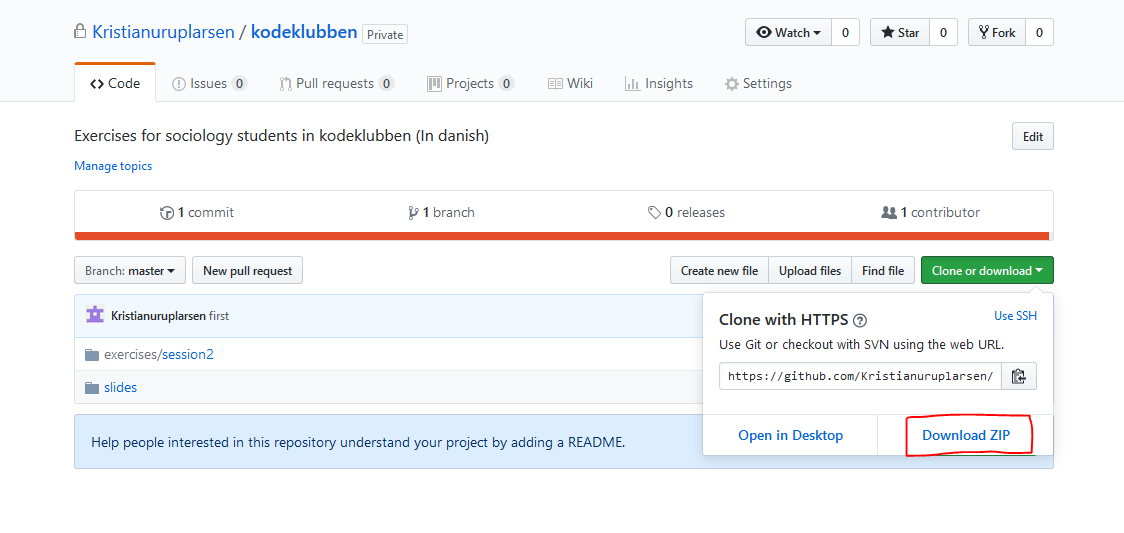
\includegraphics[width=\textwidth]{figs/setup.PNG}
\end{figure}
\end{frame}

\begin{frame}[fragile]{Sidste gang}
Sidste gang downloadede og rensede vi et datasæt over danske kommunalpolitikeres holdninger:
\begin{itemize}
  \item Åben det datasæt i selv gemte sidste gang, eller
  \item Hent datasættet online:
  \begin{lstlisting}[language=python]
import pandas as pd

url = 'https://raw.githubusercontent.com/'\
      'Kristianuruplarsen/kodeklubben/master/'\
      'data/candidates.csv'
df = pd.read_csv(url)
  \end{lstlisting}
\end{itemize}
\end{frame}

\begin{frame}[fragile]{Projektet}
\textcolor{gray}{Sidste gang:}
\begin{itemize}
  \item[\textcolor{gray}{$\bullet$}] \textcolor{gray}{Download data fra DR}
  \begin{itemize}
    \item[\textcolor{gray}{$\bullet$}] \textcolor{gray}{internet-hacks}
    \item[\textcolor{gray}{$\bullet$}] \textcolor{gray}{Interagere med nettet gennem python}
  \end{itemize}
  \item[\textcolor{gray}{$\bullet$}] \textcolor{gray}{Rens datasættet og gør klar til alt det sjove}
  \begin{itemize}
    \item[\textcolor{gray}{$\bullet$}] \textcolor{gray}{jonglere med data og formatter}
  \end{itemize}
\end{itemize}

Denne gang:
\begin{itemize}
  \item Alt det sjove.
  \begin{itemize}
    \item \textit{Dimensionality reduction}
    \item Interaktive plot
  \end{itemize}
\end{itemize}
\end{frame}





\section{Øvelser}

\end{document}
